\documentclass{article}

\usepackage[margin=.75in]{geometry}
\usepackage{graphicx}
\usepackage{placeins}
\usepackage{listings}

\lstset{breaklines=true}
\graphicspath{{diagrams/},{afit-images/}} 

\begin{document}

\section{Network Setup}
\subsection{Software}
\par Testing was done on a network of seven physical servers. Each uses Ubuntu 12.04 with the following software installed (these include the tools necessary for compilation):

\begin{itemize}
\item gcc $>=$4
\item linux-headers 3.5.0
\item Autoconf $>=$2.69
\item Automake $>=$1.11
\item libtool $>=$2.4.2
\item libpcap-dev $>=$1.3.0
\item libpolarssl-dev $>=$1.1.4
\item libpthread-dev $>=$ 1.1.1 
\item tcpdump
\item python 2.7
\item python-scapy $>=$ 2.2.0
\end{itemize}

\par To install these in Ubuntu:
\begin{lstlisting}
$ sudo apt-get install automake autoconf build-essential libtool libpcap-dev libpolarssl-dev python-libpcap python-scapy
\end{lstlisting}

\par Each host should have SSH private key login turned on and \texttt{sudo} should be allowed without a password for all commands.

\subsection{Layout}
\par The seven systems are arranged into the network shown in Figure \ref{fig:layout}. IPs and masks are shown in this diagram as well. The precise IPs on the interfaces for the gateways are not important for test purposes, only that they fall within the given range.

\begin{figure}
\caption{Test network}
\label{fig:layout}
\centering
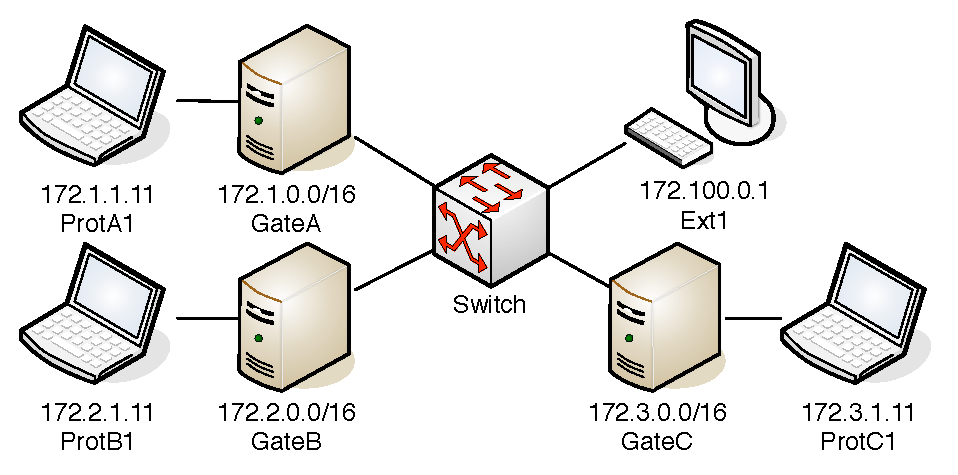
\includegraphics[width=\textwidth]{thesis_network}
\end{figure}

\par Additionally, each host (clients and gateways) have a second/third connection to a control network. This interface is used for remote management and test automation. Network routes should be configured to ensure traffic goes out the proper interfaces. In Ubuntu, \texttt{/etc/network/interfaces} should allow this to be done fairly easily with the \texttt{up route add} directive.

\subsection{Interfaces}
\par Test scripts assume \texttt{eth0} is the control network on all hosts. For clients, \texttt{eth1} is the test interface. For gateways, \texttt{eth1} should be the interface connected to the other gateways (the switch in Figure \ref{fig:layout}) and \texttt{eth2} is the interface connecting to their respective clients.

\subsection{Host Names}
\label{sec:hostnames}
\par Host name should follow those given in Figure \ref{fig:layout}, with the first letter lowercase. That is, there should be a \texttt{gateA}, \texttt{gateB}, \texttt{gateC}, \texttt{protA1}, \texttt{protB1}, \texttt{protC1}, and \texttt{ext1}.

\section{Running Experiments}
\par The file \texttt{scripts/executer.sh} controls the tests and test hosts. The hosts should have their hosts file edited to point to the hosts using the same host names as listed in Section \ref{sec:hostnames}. Running \texttt{executer.sh} without any commands will display the available commands. To run tests, \texttt{executer.sh start-tests} will run all tests.

\par \texttt{executer.sh} also includes several configurable values at the top of the file. Most important is setting the \texttt{LOCAL} host name to the controlling machine's name (used to allow the script to determine if it is running on the test network or controller machine). Secondly, \texttt{RESULTSDIR} should be set to where test logs should be saved.

\section{Processing Runs}
\par After experiments have been run, \texttt{executer.sh process-runs} will push the results back out to the test network to be processed in parallel by \texttt{scripts/process\_run.py}. As each completes, a database with the results will be pulled back to each run's directory. \texttt{process\_run.py} may also be called directly to process individual runs, see \texttt{process\_run.py --help} for more information).

\section{Producing Graphs}
\par After all experiments are processed (they have a run database file), \texttt{scripts/consolidate\_data.py} will produce a CSV file with all numbers. By placing this file alongside the thesis as \texttt{results.csv}, rebuilding the thesis will generate new graphis in the PDF. R code to produce them is given in \texttt{chapter5.Rnw}.

\end{document}

